\section{Zentraler Grenzwertsatz}
$\mu \sigma^2$ bekannt aber nicht die Verteilung
\subsection{ZGWS}
Seien $ X_{i} (i=1, ..., n)$ unabhängige identische verteilte \textbf{(i.i.d)} ZV mit Erwartungswert $\mu$ und Varianz
$ \sigma^2 $. Dann gilt für hinreichend große n ( >30) und $\overline{X} = \frac{1}{n} \sum_{i=1}^{n}$ näherungsweise:\\
$\sum_{i=1}^{n} X_{i}  \thicksim  N_{n\mu, n\sigma^2}$  \&\\
%bezieht sich auf $X_{i}$\\
$\frac{\sum X_{i}-n\mu}{\sqrt{n}\cdot \sigma} \thicksim N_{0,1} $\\
$\sum X_{i} $ bezieht sich auf Y; $\sum X_{i} - n\mu$ bezieht sich auf $ X_{i}$; 
$ \overline{X} \thicksim N_{\mu, \frac{\sigma^2}{n}} $ \& $ \frac{\overline{X}-\mu}{\sigma} \thicksim N_{0,1} $; 
Der Satz gilt sogar allgemeiner, wenn die $X_{i}$ abhängig und nicht identisch verteilt sind, vorausgesetzt kein $ X_{i} $ ist deutlich dominanter?! als die anderen.Für die Voraussetzung des  ZGW ist, dass die $ X_{i} $ nicht normalverteilt sein müssen., damit $\sum_{i=1}^{n} X_{i}$ oder $\overline{X}$  bei \textbf{hinreichend großem n} normalverteilt sind. Faustregel: \textbf{Je} schiefer die Verteilung der $ X_{i}$ , \textbf{desto} größer muss n sein: 
\textbf{n>30}: falls die unbekannte Verteilung ohne markanten Ausreißer, aber schief ist (Exponentialverteilung); 
\textbf{n>15:} falls die unbekannte Verteilung annähernd symmetrisch ist(Binomialverteilung); 
$ \boldsymbol{ n \le 15 }$: falls die unbekannte Verteilung annähernd normalverteilt ist; 
\subsection{$\phi$}
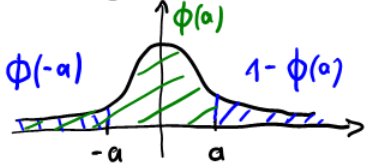
\includegraphics[scale=0.25]{./pic/ZGWPhiVerteilung.png} $ \phi(-a ) = 1 - \phi(a) $; $\phi(a) = 1-\phi(-a) $; 
$ P(-a < Z < a) = \phi(a) - \phi(-a) = \phi(a) - (1-\phi(a)) = \underline{ 2\phi(a) -1 } $ or $ 1-\phi(-a) - \phi(-a) = 1 -2\phi(-a)$
\subsection{$\phi^{-1}$}
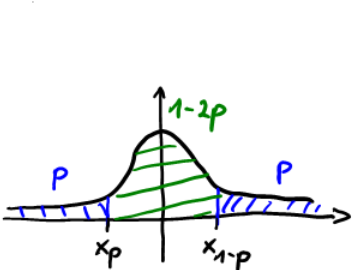
\includegraphics[scale=0.25]{./pic/ZGWPhi-1Verteilung.png}
$  -x_{p} = x_{1-p} \Leftrightarrow -qnorm(p) = qnorm(1-p) \Leftrightarrow -\phi^{-1}(p) = \phi^{-1}(1-p) $
\textbf{Zusammenhang}
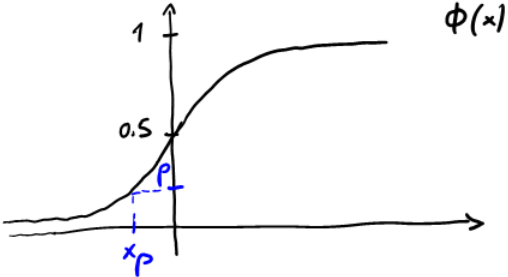
\includegraphics[scale=0.25]{./pic/ZGWSigmoidFunction.png} $ \phi^{-1}(p) = x_{p} $; 
\textbf{Aufgabentypen:} 
Seien $ X_{i} $ i.i.d. ZV mit $\mu$ und $ \sigma^2 $, aber unbekannter Verteilung. Dann sind $ Z_{1} = \frac{\sum X_{i}-n\mu}{\sqrt{n}\sigma}$ und $Z_{2} = \frac{\overline{X}-\mu}{\sigma} $  näherungsweise standardnormalverteilt.\\
	$\circ$ Es lassen sich Wahrscheinlichkeiten für $\sum X_{i}, \overline{X}, Z_{1}$ oder $ Z_{2} $ berechnen.\\
	$\circ$ Es lässt sich \textcolor{red}{n} bestimmen, so dass, zu vorgegebener Schranke $ k $ und Wahrscheinlichkeit $ p $ gilt: $ P(Z_{i} > k) \geq p $ or $ P(-k \leq Z_{i} \leq k) \geq p $
\subsection{Stichprobenvert.normalvert.\\Grundgesamt.}
\subsection{Stichprobenmittel}
Die Stichprobenfunktion $ \overline{X} = \frac{1}{n} \sum_{i=1}^{n} X_{i} $ ist eine erwartungstreue Schätzfunktion für Erwartungswert $ \mu $, d. h.$E[\overline{X}] = \mu$
\subsection{Stichprobenvarianz}
Die Stichprobenfunktion $ S^2 = \frac{1}{n-1} \sum_{i=1}^{n} (X_{i} - \overline{X})^2 = \frac{1}{n-1}(\sum_{i=1}^{n}X_{i}^2 - n\overline{X}^2)$ist eine erwartungstreue Schätzfunktion für die Varianz $\sigma^2$, d. h. $E[S^2] =\sigma^2$; 
$ E[\overline{X}] = E[\frac{1}{n}\sum X_{i}] = \frac{1}{n} E[\sum X_{i}] = \frac{1}{n} \sum_{i=1}^{n} E[X_{i}] = \frac{1}{n} n\mu = \mu$; 
$ Var[\overline{X}] = Var[\frac{1}{n}\sum X_{i}] = \frac{1}{n^2} Var[\sum X_{i}] = \frac{1}{n^2}n\sigma^2 = \frac{\sigma^2}{n} $; 
Seien $ X_{i} (i=1, ..., n)$ unabhängige normalverteilte ZV mit Erwartungswert $\mu$ und Varianz $\sigma^2$. Dann gilt:
\textbf{bei bekannter Varianz:} $ \frac{\overline{X} -\mu}{\sigma} \sqrt{n} \thicksim N_{0,1}$; 
$ \frac{(n-1)S^2 = \sum(x-\overline{x})^2}{\sigma^2 \Rightarrow \text{Standardisierung}} \thicksim \chi_{n-1}^{2}$; 
\textbf{Bei unbekannter Varianz:} $ \frac{\overline{X}-\mu}{S}\sqrt{n} \thicksim t_{n-1}$; 